\chapter{Achtergrond datastores}
\label{cha2}

Sinds de jaren '70 zijn zogenaamde \textit{relational database management systems} (kortweg RDBMS) de voornaamste technologie voor de grootschalige opslag van gegevens. Ze zijn gestoeld op 2 belangrijke principes, namelijk het relationele datamodel \cite{codd1970relational} en de gestructureerde querytaal SEQUEL, beter gekend als SQL \cite{chamberlin1974sequel}. De architectuur van vele RDBMS is nog steeds gebaseerd op de eerste implementatie van een dergelijk systeem, namelijk het IBM onderzoeksproject System R \cite{blasgen1981system}, ook uit halverwege de jaren '70 \cite{Stonebraker:2007:EAE:1325851.1325981}. System R is uiteraard ontworpen voor destijds relevante hardwarekarakteristieken en productvereisten: business data processing via een command line interface, en dit op computersystemen met trage processoren, kleine werk- en schijfgeheugens maar relatief grote bandbreedte tussen de schijfopslag en het werkgeheugen. Dit leidde tot een aantal architecturale features die nog steeds terug te vinden zijn in hedendaagse RDBMS:
\begin{itemize}
\item Disk-geori\"enteerde opslag- en indexstructuren
\item Multithreading om latency te verbergen
\item Concurrency-controlemechanismen op basis van locking
\item Log-gebaseerd herstel van fouten
\end{itemize} 
Ondanks gigantische technologische vooruitgang op gebied van hardware en sterk gediversifieerde gebruiksscenario's, is er sinds hun ontstaan 40 jaar geleden weinig drastisch veranderd aan het concept van de RDBMS en zijn deze systemen de werkpaarden van de industrie geworden op het vlak van dataopslag.\\

Beginnende in de jaren 2000 groeide in de IT-wereld dan ook het besef dat de rigide \textit{one size fits all}-aanpak van RDBMS voor vele moderne toepassingen achterhaald dreigde te geraken. Met grote opkomende spelers uit de web-industrie zoals Google, Amazon en Facebook aan het roer leidde dit tot de opkomst van de NoSQL-beweging. NoSQL staat, in tegenstelling tot wat de naam doet vermoeden, voor \textit{Not only SQL} en omvat een waaier van uiteenlopende alternatieve gegevensopslagsystemen die elk in bepaalde specifieke opzichten meerwaarde trachten te bieden ten opzichte van het klassieke relationele systemen. In tegenstelling tot de 'Zwitsers zakmes'-aanpak van RDMBS, leggen ze zich toe op zeer gespecialiseerde toepassingsdomeinen en proberen daarin relationele systemen te overtreffen. Vaak betekent dit dat NoSQL systemen vele voor hun doel onnodig geachte features van SQL systemen achterwege laten, of afzwakken. Een goed voorbeeld hiervan zijn de ACID-eigenschappen uit het relationele model die in vele NoSQL-systemen gereduceerd zijn tot zogenaamde BASE-eigenschappen (op het verschil tussen beide komt sectie \ref{consistentie} nog uitgebreid terug).

De reden waarom web-spelers overstapten op NoSQL-systemen of er zelf ontwierpen, is voornamelijk dat deze geschikter zijn voor de enorme hoeveelheden data die dergelijke bedrijven sinds de opkomst van Web 2.0 moeten verwerken. NoSQL-systemen staan er om bekend horizontaal en incrementeel te schalen naar gigantische datasets: door eenvoudigweg servers toe te voegen aan het cluster onder de databank, en niet door bestaande servers up te graden (i.e. verticaal schalen), kan een cluster vlot meegroeien met de dataset. Bovendien draaien NoSQL-systemen doorgaans op goedkope commodity hardware, dus standaard servers, in plaats van dure gespecialiseerde databankservers. Goedkope doordeweekse servers laten toe om zowel kost- als energie-effici\"enter redundantie en dus ook fouttolerantie in te bouwen en zo de zeer hoge vereiste beschikbaarheid te garanderen \cite{barroso2003web}. NoSQL-systemen zijn bijgevolg grootschalige, gedistribueerde systemen, met bijhorende mechanismen om data ten eerste op te splitsen en te verspreiden (ook: partitioneren of sharden) en ten tweede te repliceren over het cluster. Replicatie heeft meerdere doelen: verhoogde bedrijfszekerheid, load balancing en verhoogde doorvoer in lees-intensieve toepassingen.

\section{Concepten}

Deze sectie belicht de belangrijkste begrippen in verband met NoSQL-databanken en contrasteert waar nodig met gelijkaardige concepten in het klassieke traditionele model.

\subsection{Partitionering}

Gezien de grote datahoeveelheden en gedistribueerde setting van NoSQL is het een noodzaak data in de databank te verspreiden. Er bestaan meerdere strategie\"en om de entries in een databank (dit kunnen rijen, documenten, simpele values,\ldots zijn) over de nodes in een cluster te verdelen. Ten eerste is er het onderscheid tussen horizontaal en verticaal partitioneren: bij horizontaal schalen, ook sharding genoemd, wordt een entry niet gefragmenteerd, maar in zijn geheel toegewezen aan een node, op basis van een op de entry gedefinieerde key. De meeste NoSQL datastores implementeren een versie van horizontaal partitioneren. Verticaal partitioneren stamt uit het relationele model, en betekent het splitsen van grote tabellen in meerdere kleinere tabellen.\\
Binnen het horizontaal partitioneren bestaan 2 voorname methodes \cite{grolinger2013data}:
\begin{itemize}
\item \textit{Range partitioning:} elke server is verantwoordelijk voor een bepaald bereik van key-waarden. Deze methode leent zich uitstekend tot het verwerken van range queries, gezien opeenvolgende keys vaak op eenzelfde node zullen liggen. Er is echter ook een belangrijk nadeel met deze aanpak verbonden: ze kan leiden tot load-balanceringsproblemen en \textit{hot spots}. Wanneer een applicatie bijvoorbeeld de gegevens in volgorde van hun key-waarden verwerkt, zal de werklast steeds bij dezelfde servers geconcentreerd liggen. Een ander nadeel is dat een centrale routing server de mapping van de ranges van keys naar nodes moet bijhouden, die dan client requests naar de juiste nodes door kan sturen. Dit introduceert een mogelijke flessenhals in het systeem.
\item \textit{Consistent hashing:} zoals de naam doet vermoeden, gebeurt de partitie in dit geval op basis van een hash van de key van entries. De output van de hash-functie wordt als een ring beschouwd en alle nodes krijgen een willekeurige waarde of positie toegewezen op deze ring. Een entry wordt dan toegewezen door via de hash van zijn key zijn positie in de ring te bepalen en vervolgens de ring klokwijs te bewandelen tot de eerste node met positie groter dan de positie van de entry. Het voordeel van consistent hashing is dat de positie van een object zeer snel berekend kan worden en dat hier geen centraal bewaarde mapping voor nodig is. Bovendien is het toevoegen van nodes zeer eenvoudig: enkel de buren van een nieuwe node op de ring merken dit, waardoor weinig entries verplaatst moeten worden. Een belangrijk nadeel is dat consistent hashing range queries bemoeilijkt, gezien opeenvolgende entries nu verspreid kunnen liggen over verschillende nodes.\\
Een techniek die vaak gepaard gaat met consistent hashing is het gebruik van \textit{virtual nodes} om load-balancing te verbeteren: elke fysieke node in het cluster krijgt meerdere posities toegewezen op de ring, en is zo verantwoordelijk voor meerdere virtuele nodes. Dit zorgt voor een betere verdeling van de entries over de nodes, gezien entries niet per se uniform over de ring verdeeld liggen. Bovendien moeten niet alle fysieke nodes verantwoordelijk zijn voor evenveel virtuele nodes: het systeem kan meer virtuele nodes toewijzen aan performantere fysieke nodes en zo rekening houden met heterogeniteit in de fysieke infrastructuur. Bovendien zal, bij het falen van een fysieke node, zijn opgeslagen last eerlijk verspreid worden tussen de overgebleven fysieke nodes. Omgekeerd zal een nieuwe node wanneer hij toetreedt tot het cluster van alle andere fysieke nodes ongeveer evenveel last overnemen  \cite{grolinger2013data}\cite{decandia2007dynamo}.
\end{itemize}  

\subsection{Consistentie}
\label{consistentie}

Consistentie van database-transacties betekent dat transacties de databank in een consistente staat achterlaten: alle data die een applicatie kan zien, is een consistente snapshot van de databank \cite{ports2010transactional}. Traditionele RDBMS bieden vaak transacties met de zogenaamde ACID-eigenschappen \cite{haerder1983principles}:
\begin{itemize}
\item \textbf{Atomicity:} Elke transactie gebeurt ofwel volledig, ofwel helemaal niet.
\item \textbf{Consistency:} Elke transactie laat de databank in consistente staat achter.
\item \textbf{Isolation:} Elke transactie verloopt volledig ge\"isoleerd van elke andere transactie en be\"invloedt deze dus op geen enkele manier.
\item \textbf{Durability:} Eens voltrokken, blijft elke transactie duurzaam bewaard in de databank, ook in het geval van stroomonderbrekingen, crashes of fouten.
\end{itemize}

Zoals Eric Brewer stelde in zijn bekende CAP-theorema \cite{brewer2000towards}, is het in een gedistribueerd systeem niet eenvoudig zowel consistentie, availability als tolerantie voor partities te bereiken en zijn 2 van deze 3 eigenschappen het hoogst haalbare\footnote{Brewer kwam hier zelf 12 jaar later op terug, stellende dat mits goede omgang met partities het toch mogelijk is een trade-off van alle drie te bereiken \cite{brewer2012cap}.}.
Ook in NoSQL-systemen, die vaak gedistribueerd van aard zijn, is het garanderen van consistentie geen triviale opgave. Afhankelijk van de gehanteerde schrijfstrategie is het mogelijk dat verschillende knopen in het cluster verschillende versies van data zien, als updates nog niet in het volledige cluster doorgekomen zijn. Daarom is er het onderscheid tussen strikte en uiteindelijke ("\textit{eventual}") consistentie: strikte consistentie is de gekende vorm waarin updates onmiddellijk zichtbaar zijn op alle nodes in het cluster, en dus ook naar bovenliggende applicaties toe. In het geval van uiteindelijke consistentie garandeert het systeem enkel dat na verloop van tijd alle nodes in het cluster dezelfde, up-to-date versie van de data zullen zien. NoSQL-systemen bieden dan ook vaak de BASE-eigenschappen, een zwakkere versie van de ACID-garanties:
\begin{itemize}
\item \textbf{Basically available:} Het systeem is onder quasi alle omstandigheden beschikbaar.
\item \textbf{Soft state:} Het systeem verkeert niet altijd in een consistente staat
\item \textbf{Eventually consistent:} Na verloop van tijd zal het systeem in een gekende staat verkeren.
\end{itemize}

Vele NoSQL-systemen stellen de gebruiker echter niet voor een voldongen feit bij de keuze tussen strikte en uiteindelijke consistentie: dankzij zogenaamde \textit{quora} kan de gebruiker zelf configureren welke consistentie het systeem levert. Door lees- en schrijfquora in te stellen, kan de gebruiker tunen hoeveel replica's respectievelijk moeten returnen bij een schrijfopdracht, en het welslagen van een schrijfopdracht moeten bevestigen. Op deze manier kan de gebruiker zelf een trade-off maken tussen snel lezen, schrijven en de behaalde consistentie. Bovendien zal de gebruiker, wanneer de som van het lees- en schrijfquorum groter is dan de replicatiefactor van het cluster, steeds de meest recente versie van gegevens zien, wat hetzelfde betekent als onmiddellijke, strikte consistentie.

\subsection{Storage layout}
Ook op het gebied van hoe ze gegevens zowel op schijf als in het geheugen opslaan, verschillen NoSQL-systemen van elkaar. Sommigen hanteren de gebalanceeerde B-bomen die ook vele RDBM-systemen gebruiken. Anderen, in navolging van Google Bigtable, doen beroep op zogenaamde \textit{log-structured merge trees}. In deze strategie worden updates niet onmiddellijk naar schijf geschreven: de data wordt in werkgeheugen aangepast en de update wordt op schijf gelogd. Wanneer er genoeg updates in geheugen gebeurd zijn, worden deze allemaal tegelijkertijd naar schijf geschreven. Dit kan sequentieel gebeuren, en vermijdt zo vele random writes, wat de schrijfdoorvoer uiteraard ten goede komt. 


\section{NoSQL-klassen}

NoSQL databanken zijn er in verschillende soorten en kunnen op basis van hun datamodel in een aantal categorie\"en onderverdeeld worden:

\begin{itemize}
\item \textbf{Key-Value stores} Deze zijn vergelijkbaar met dictionaries en mappen unieke keys op values. Deze values zijn voor de databank volledig betekenisloze byte-arrays en de enige manier om ze op te vragen, is via de bijhoren key. Voor zeer eenvoudige toepassingen resulteert dit in hoge lees- en schrijf-throughput, maar meer geavanceerde features zoals indexing, queries, en het modelleren van relaties binnen de data zijn hierdoor niet mogelijk\cite{hecht2011nosql}\cite{grolinger2013data}.

\item \textbf{Columnar stores} Deze zijn gebaseerd op het datamodel dat Google's Bigtable heeft ge\"introduceerd en slaan data op in een spaarse, gedistribueerde, persistente en multidimensionele gesorteerde map\cite{chang2008bigtable}. In het geval van Bigtable zijn dit drie dimensies: row key, column key en een timestamp. Omdat ook hier het systeem de opgeslagen data niet interpreteert, is het modelleren van relaties niet op een effici\"ente manier mogelijk. Dit wordt overgelaten aan de bovenliggende applicatie\cite{hecht2011nosql}.

\item \textbf{Document stores} Deze bewaren data als key-value paren en encapsuleren deze in documenten. Values kunnen van een brede waaier aan types zijn, zoals geneste documenten, lijsten of scalars. De namen van attributen kunnen dynamisch gespecifieerd worden tijdens runtime en moeten geen vooraf vastgelegd schema volgen\cite{cattell2011scalable}. Dit is geschikt voor het modelleren van ingewikkelde datastructuren. Vele document stores gebruiken het JSON-bestandsformaa (of een daarvan afgeleide vorm). In tegenstelling tot columnar stores, zijn de waarden in documenten niet betekenisloos voor het document store systeem en het is dus mogelijk hier indexen op te defini\"eren en queries op uit te voeren\cite{hecht2011nosql}.

\item \textbf{Graph databases} Zoals de naam doet vermoeden, stammen deze uit grafentheorie en maken ze gebruik van grafen als datamodel. Ze zijn uitermate geschikt om sterk verweven data te beheren, van bronnen zoals sociale netwerken of location based services. Hiervoor doen ze beroep op effici\"ente mechanismen om grafen te doorlopen waar andere systemen kostelijke operaties als recursieve joins gebruiken\cite{hecht2011nosql}.

\end{itemize}

De term NewSQL slaat op een verzameling systemen die ambi\"eren het klassieke relationele datamodel te combineren met de schaalbaarheid, distributie en fouttolerantie van NoSQL systemn. Hoewel ze allen de gebruiker het relationele model en SQL-achtige query mogelijkheden bieden, verschillen NewSQL stores onderling grondig, afhankelijk van de onderliggende architectuur. Zo zijn er onder meer systemen die gebouwd zijn bovenop bestaande NoSQL databanken, en andere die alle data in main memory opslaan.\cite{grolinger2013data}

\section{NoSQL: vergelijkende studie}
\label{nosql_survey}

Op de vraag of NoSQL en NewSQl-systemen al dan niet geschikt zijn om het genoomanalyseproces schaalbaarder te maken, bestaat geen eenvoudig antwoord. Gezien de grote diversiteit in de beschikbare gegevensopslagsystemen, zullen sommige systemen onvermijdelijk beter geschikt zijn dan andere, of beter geschikt voor andere aspecten van de genoom-analyse pipeline. Een vergelijkende studie van NoSQL- en NewSQL-systemen dringt zich dus op. Deze sectie bekijkt 6 systemen in meer detail en licht toe hoe ze van pas zouden kunnen komen in de genoomanalyse.

\subsection{Methodologie}

Omwille van het enorme aanbod aan NoSQL en NewSQL systemen was een exhaustieve studie niet haalbaar. Deze vergelijkende studie behandelt de populairste datastores in een aantal relevante categorie\"en, namelijk document stores, columnar stores en NewSQL stores. Key-value stores en graph databases komen niet aan bod, aangezien hun datamodellen niet geschikt zijn voor de toepassing in kwestie. De uiteindelijke selectie werd gemaakt volgens criteria vergelijkbaar met die in \cite{grolinger2013data}, met de ranking van DB-Engine Ranking \cite{db_engine_rank} als maat voor de populariteit.\\

Deze ranglijst tracht populariteit te meten op basis van enkele parameters, zoals aantal vermeldingen op websites, algemene interesses volgens Google Trends, frequentie van technische discussies op fora zoals StackOverflow, vacatures i.v.m. de technologie en vermeldingen in professionele profielen op sites zoals LinkedIn. De resulterende selectie bestaat uit de document stores MongoDB en CouchBase Server, wide columnar stores Cassandra en HBase en NewSQL database VoltDB. Er bestaat al een uitbreiding van de DNA sequencing pijplijn die het ExaScience Life Lab gebruikt om MongoDB  databanken als in- en/of uitvoer te gebruiken voor de pijplijn. Dit maakt MongoDB uiteraard nog relevanter. Ten laatste werd ook NewSQL query engine Cloudera Impala in de studie betrokken wegens expliciete interesse van onderzoekers in het eerder vernoemde lab.

\begin{landscape}
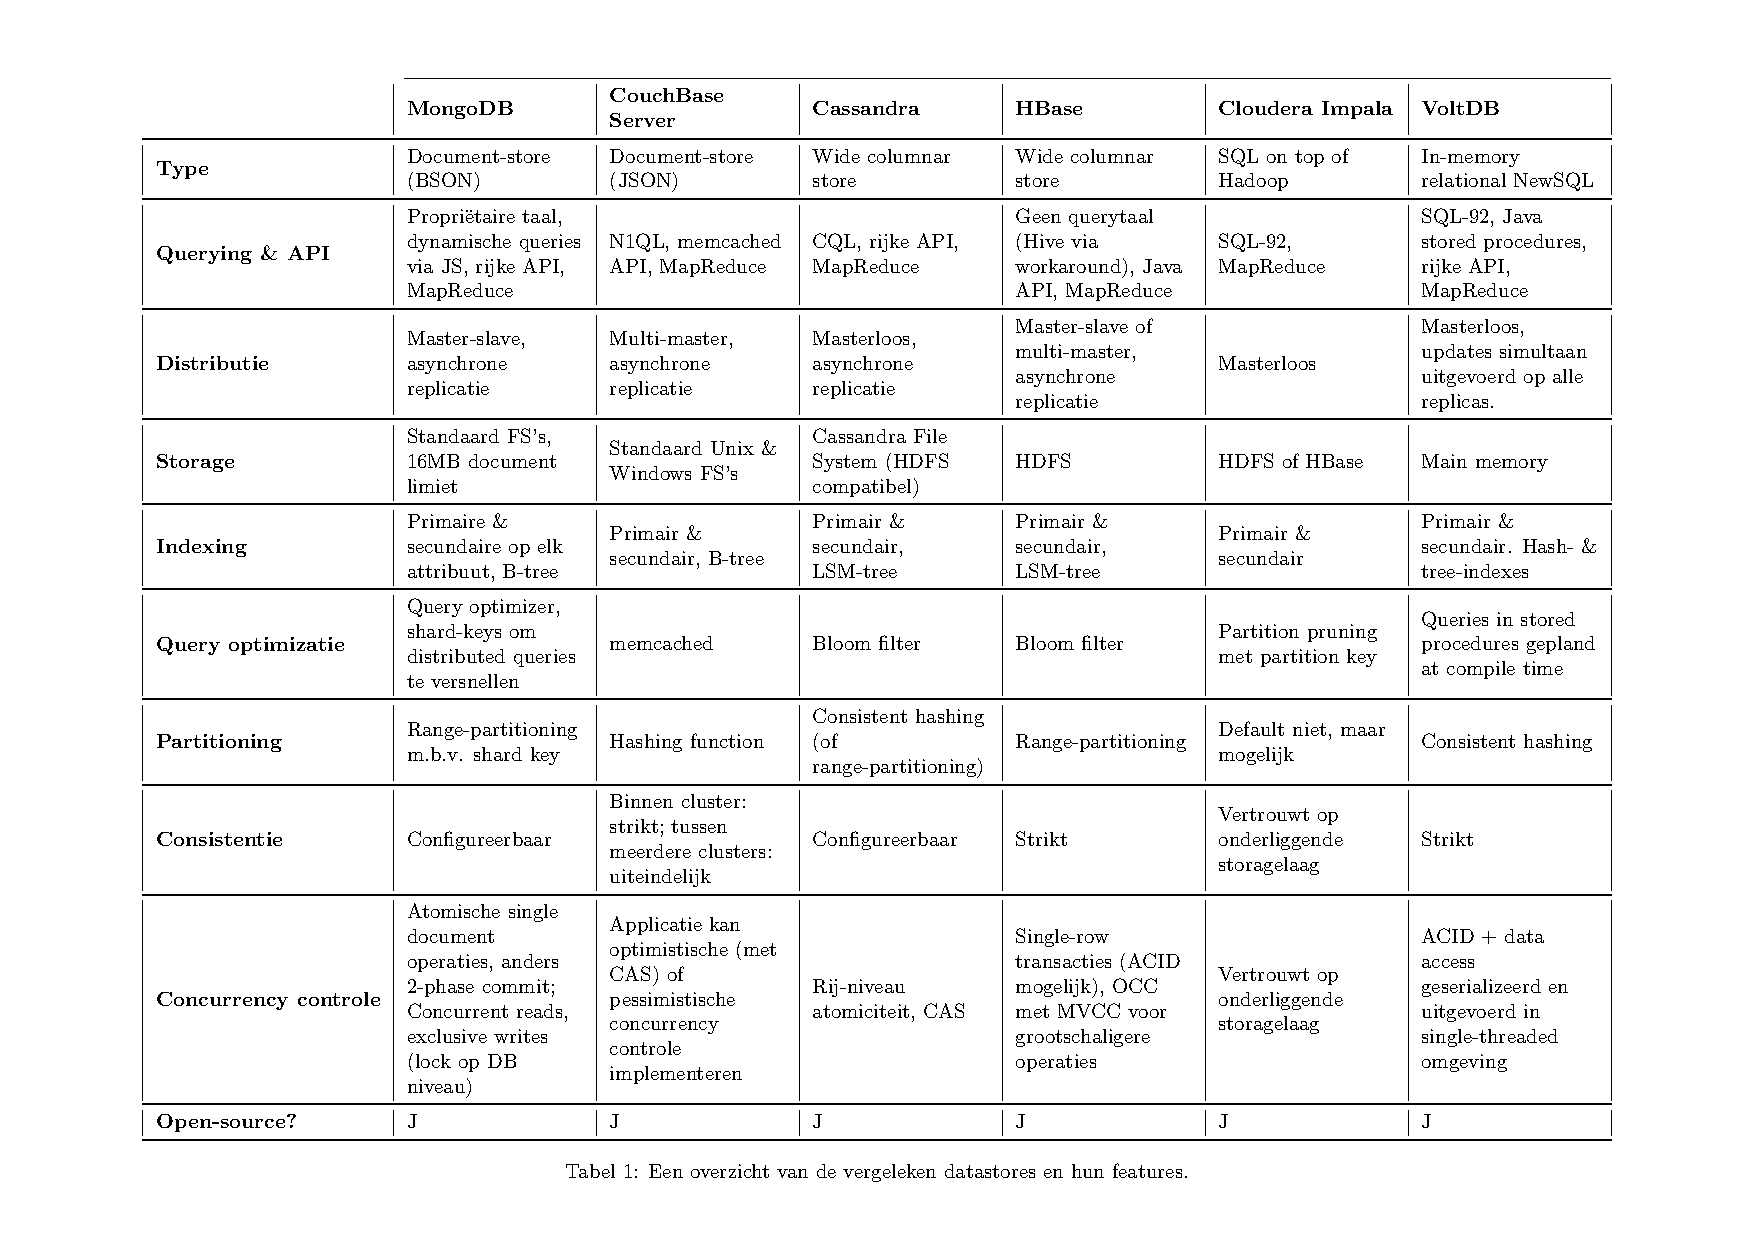
\includepdf[angle=90]{NoSQL_table_nl.pdf}
\label{survey_tabel}
\end{landscape}

\noindent Deze 6 systemen vergeleek ik 
%TODO ik?
vervolgens op een aantal voor high performance computing relevante eigenschappen zoals indexeringsmechanismen, interfaces naar de gebruiker en API's, distributiestrategie, concurrency controle en consistentiemodel. Tabel \ref{survey_tabel} geeft een overzicht weer van de bestudeerde systemen.



\subsection{Document stores}

\subsubsection{MongoDB}

MongoDB slaat gegevens op in BSON (binary JSON) documenten. Het systeem biedt krachtige ondersteuning voor indices, vooral door de mogelijkheid om secundaire indices van een brede waaier van types te defini\"eren op alle attributen, zoals in het relationele model. Deze indices zijn gebouwd op B-trees \cite{mongodb_indexes}. Om denormalizatie te bevorderen, kunnen documenten geneste documenten en arrays bevatten. Zo zijn joins ook overbodig in de query taal.\\
De bestandsgrootte is beperkt tot 16 MB, om te voorkomen dat \'e\'en enkel document buitensporig veel RAM of bandbreedte opeist. Om grotere bestanden te bewaren, kan het ingebouwde GridFS (dat integenstelling tot wat de naam doet vermoeden, geen volwaardig file system is) automatisch bestanden opsplitsen in kleinere delen en deze delen als aparte documenten bewaren, zonder dat de gebruiker zich hierom moet bekommeren.\\
MongoDB biedt API's in zeer vele programmeertalen en de functionaliteit om het equivalent van SQL \texttt{WHERE}-clausules te defini\"eren als javascript uitdrukkingen. MongoDB vertaalt deze vervolgens naar een eigen, interne en afgeschermde query taal \cite{grolinger2013data}. De query optimizer van MongoDB verwerkt queries en kiest voor elke query een zo effici\"ent mogelijk uitvoeringsplan gegeven de beschikbare indices. Deze plannen worden gecached als er meerdere goede alternatieven zijn en kunnen geherevalueerd worden naarmate de gegevensset in de databank evolueert.\\
Qua consistentie laat MongoDB de keuze tussen uiteindelijke en strikte consistentie. Strikte consistentie is mogelijk door ofwel enkel te lezen van de master node (die de meest up-to-date versie van de data heeft) of na schrijfopdrachten te wachten tot alle replica's bevestigd hebben alvorens verder te gaan. De eerste optie introduceert een bottleneck bij het lezen van data, de tweede verhoogt de latentie van schrijfopdrachten.\\
MongoDB repliceert data asynchroon en partitioneert in ranges: nodes zijn verantwoordelijk voor ranges van keys. Dit zorgt voor snelle range queries, maar kan hotspots en load-balancingproblemen veroorzaken. Dankzij een master-slave struktuur kan MongoDB updates gemakkelijk naar de juiste replica's doorverwijzen.
Op het gebied van concurrency controle biedt MongoDB atomiciteit binnen documenten en reader-writer locks. Bij schrijfopdrachten de databank locken heeft een zware impact op de performantie in scenario's waar veel geschreven moet worden.\\\\
Kortom, MongoDB bewaart BSON-bestanden op een zeer toegankelijke manier met flexibele query- en indexeringsmechanismes. De concurrency- en consistentiemodellen daarentegen vertonen enkele nadelen.

\subsubsection{Couchbase Server}

Couchbase, het resultaat van de fusie tussen CouchDB en Membase, slaat gegevens op in JSON documenten. Het hanteert het memcached protocol om een gedistribueerde cache en is bedoeld voor zeer interactieve toepassingen met hoge vereisten op gebied van latentie \cite{grolinger2013data}\cite{couchbase_about}.
De JSON documenten kunnen genest zijn en kunnen doorzocht worden met een uitgebreide, SQL-achtige taal, N1QL (op het moment van schrijven is dit wel nog steeds een developer preview, uitgebracht in januari 2015) \cite{couchbase_n1ql}.
Net als MongoDB kunnen primaire en secundaire indices gedefinieerd worden en zijn deze gestoeld op B-trees \cite{couchbase_index}.\\
Binnen \'e\'en cluster zijn transacties strikt consistent, maar tussen meerder clusters slechts uiteindelijk consistent.\\
CouchBase biedt gebruikers de keuze tussen optimistische (m.b.v. compare-and-swap) en pessimistische (m.b.v. 'finegrained locking') concurreny controle.\\\\
Dankzij zijn flexibele datamodel, caching en concurrency controle, past CouchBase goed voor toepassingen die snelle en intensieve interactieve vergen tussen gebruiker en data.

\subsection{Columnar stores}

\subsubsection{Cassandra}

Cassandra werd oorspronkelijk ontwikkeld voor intern gebruik bij Facebook maar is later als Apache opensourceproject publiekelijk beschikbaar gemaakt. Het combineert het datamodel van Google's Bigtable systeem met de architectuur en distributiestrategie van Amazons DynamoDB. Het is gericht op flexibele, quasipermanent beschikbare opslag van zeer grote datasets op goedkope standaardhardware, met daarenboven hoge througput voor schrijfopdrachten zonder effici\"entie bij leesopdrachten op te offeren \cite{borthakur2011apache}.\\
Sinds zijn ontstaan is Cassandra wel op enkele vlakken afgeweken van het BigTable-model \cite{cassandra_then&now}, in die zin dat het nu tabellen en samengestelde kolommen
%TODO betere vertaling voor composite columns?
biedt, evenals een eigen query taal, CQL \cite{cassandra_CQL}. CQL vertoont op het gebied van syntax en functionaliteit sterke gelijkenissen met SQL, maar is toch sterk beperkt. Zo biedt het bijvoorbeeld geen \texttt{JOIN}-clausule, en zijn \texttt{WHERE}-clausules aan sterke voorwaarden onderhevig. Cassandra moedigt het samen bewaren van gegevens die samen opgevraagd worden sterk aan en ondersteunt denormalizatie met features zoals collection types.\\
Cassandra heeft indexeringsmechanismes and implementeert deze met log-structured merge trees, met hogere schrijfthroughput als gevolg.
Net als Bigtable biedt Cassandra ook Bloom filters: een effici\"ent probabilistische mechanisme om te voorspellen of een object in een verzameling zit (in dit geval, of een key in een tabel ligt, dat het aantal nodeloze table scans beduidend kan inperken \cite{mullin1983second}.\\
Om lineair in het aantal ingeschakelde nodes te kunnen schalen naar zeer grote datasets, opereert Cassandra op een volledig hi\"erarchieloze wijze. Vanuit het perspectief van het CAP-theorema, spitst Cassandra zich toe op availability en partition tolerance, ten koste van onmiddellijke consistentie. Het consistentieniveau kan wel per query door de gebruiker bepaald worden, zoals later verduidelijkt wordt. Hoge beschikbaarheid en tolerantie voor fouten bereikt Cassandra door asynchroon data te repliceren over verschillende nodes, met consistent hashing en virtuele nodes om frequent komen-en-gaan en incrementeel toevoegen van nodes op te vangen. Het aantal replica's kan de gebruiker zelf kiezen. Bovendien voorziet Cassandra ook interdatacenterreplicatie, om zelfs het falen van volledige datacenters op te vangen \cite{decandia2007dynamo} \cite{lakshman2010cassandra} \cite{cassandra_then&now}.\\
Bij lees- en schrijfopdrachten kan de gebruiker een quorum specifi\"eren. Hoewel Cassandra met uiteindelijke consistentie voor het oog ontworpen werd, is onmiddellijke consistentie mits een juiste keuze van de quorum dus ook een optie.\\
Op het gebied van concurrency controle garandeert Cassandra atomiciteit binnen rijen en serializeerbare \textit{lightweight transactions}, eigenlijk compare-and-set functionaliteit, voor grotere operaties.
\\\\
Samengevat biedt Cassandra redelijk flexibele datamodellering met (licht beperkte) query- en indexeringsmechanismen via de CQL-interface. Het sterkste punt is echter dat Cassandra incrementeel schaalt naar enorme datasets, dankzij uitvoerige replicatie- en foutverwerkingsfeatures.

\subsubsection{HBase}

Apache HBase is een opensource datastore gebaseerd op het datamodel van Google Bigtable, die draait bovenop het Hadoop Distributed File System (HDFS) in plaats van het Google File System (GFS).\\
Sinds z'n lancering heeft HBase verschillende secundaire indexeringsmechanismes verworven. Deze zijn ook gebaseerd op LSM trees en daarnaast biedt ook HBase Bloom filters \cite{borthakur2011apache}\cite{hbase_schema}. HBase heeft een Java API, maar zonder SQL-achtige geavanceerde querytaal. Hierbij moet wel opgemerkt worden dat een omweg via Apache Hive, een ander data-opslag en -analyseproject \cite{apache_hive}, en de bijhorende querytaal HiveQL dit probleem kan verhelpen. Dankzij de HDFS-fundering can HBase vlot fungeren als in- en output voor MapReduce taken.\\
HBase partitioneert data net als Bigtable in ranges en repliceert gegevens op ofwel master-slave of multi-master wijze. Leesopdrachten worden echter niet gedistribueerd: er is slechts 1 server die instaat voor elke rij. De replica's zijn enkel bestemd voor het herstellen van fouten.\\
De sterke punten van HBase zijn de sterke consistentie, een rariteit in de NoSQL-wereld, en concurrency-model: ACID transactions binnen rijen en optimistische, multi-version concurrency controle voor grootschaligere operaties \cite{hbase_acid}\cite{grolinger2013data}\cite{borthakur2011apache}.\\

Kort samengevat laat HBase gebruikers toe flexibel data te modelleren en is het systeem vooral nuttig wanneer het startpunt een dataset in HDFS is en MapReduce-compatibiliteit een prioriteit is. HBase schaalt goed naar zeer grote datasets en beschikt over uitstekende concurrency- en consistentie-eigenschappen.

\subsection{NewSQL} 

\subsubsection{VoltDB}

VoltDB is een relationele, gedistribueerde in-memory databank, die als doel heeft de garanties van klassieke SQL-stores te koppelen met de schaalbaarheid van NoSQL-systemen, en bovendien aan zeer hoge snelheden te functioneren \cite{stonebraker2013voltdb}.\\
VoltDB bewaart gegevens in het traditionele relationele model, maar gerepliceerd en gepartitioneerd (met consistent hashing) over verschillende nodes \cite{grolinger2013data}. De data is doorzoekbaar via een (groeiende) subset van SQL-92 \cite{voltdb2010voltdb}. Queries worden bij voorkeur gedefinieerd als stored procedures in Java, met daarin ingebed de SQL uitdrukkingen. Gezien de queries dan op voorhand gekend moeten zijn, leent VoltDB zich dus ook niet optimaal tot flexibele ad-hoc queries. VoltDB ondersteunt primaire en secundaire indices en laat de gebruiker de keuze tussen hash- en boomindices \cite{voltdb_indexes}. VoltDB plant en optimaliseert de queries in stored procedures offline tijdens het compileren \cite{voltdb_query_plans}.\\
Omdat VoltDB volledig op RAM geheugen vertrouwt, is het duur om te schalen naar datavolumes in de grootorde van meerdere petabytes, maar VoltDB kan data exporteren naar andere, meer geschikte databanksystemen zoals columnaire NoSQL systemen.\\
Vooral op het gebied van concurrency controle onderscheidt VoltDB zich van andere systemen: transacties voldoen aan de ACID-eigenschappen en worden simultaan op alle replica's uitgevoerd. Het geheugen is in blokken verdeeld, die elk statisch toegewezen zijn aan \'e\'en enkele, single-threaded core. Een globale controller serializeert alle transacties waarbij meerdere nodes betrokken zijn tot een sequentie van enkelvoudige transacties en voegt deze in de transaction queues van de betrokken nodes. Op deze manier maakt VoltDB locking en latching technieken overbodig. De durability uit ACID bereikt VoltDB door op regelmatige basis snapshots van de databank in het geheugen te nemen en deze op schijf op te slaan.\\

Kort samengevat is VoltDB een relationele databank in main memory die schaalt tot relatief grote datasets, met zeer snelle SQL-query-capaciteiten en ACID-transacties. Het is bijgevolg meer geschikt voor rekenintensieve toepassingen die niet overdreven veel data verwerken, maar wel zeer lage latentie vereisen.

\subsubsection{Cloudera Impala}

Cloudera Impala is een gedistribueerde SQL-machine die draait bovenop de Hadoopstack, ofwel op HDFS of op HBase \cite{cloudera_impala}. Ze is specfiek bedoeld voor analytisch gebruik, met een focus op het leveren van real-time query-capaciteiten eerder dan op hoge throughput bij schrijfopdrachten.\\
Opgeslagen data is toegankelijk via een subset van SQL-92.\\
Impala's architectuur is bijna perfect symmetrisch gedistribueerd: alle nodes voeren hetzelfde \texttt{impalad}-proces uit, dat de belangrijkste databankfunctionaliteiten verzorgt. Elke node kan als startpunt fungeren voor een query en zal vervolgens de query in kwestie co\"ordineren. Twee processen lopen daarentegen op \'e\'en enkele (niet noodzakelijk dezelfde) node in het cluster; zij staan in voor boekhoudkundige taken en doorgeven van wijzingen aan metadata doorheen het cluster \cite{impala_components}.\\
In tegenstelling tot voorgaande opties partitioneert Impala rijen niet automatisch. De gebruiker krijgt wel de keuze hiertoe, voor in het geval de hoeveelheid gegevens hierom zou vragen \cite{impala_partitioning}.\\
Impala beschikt over een zeer effici\"ente I/O-laag die schijf- en CPU-gebruik te allen tijde hoog houdt, wat resulteert in aanzienlijk snellere prestaties dan andere SQL-on-Hadoop oplossingen zoals Apache Hive \cite{floratou2014sql}. Het inherente nadeel is echter dat de volledige dataset moet passen in het totale werkgeheugen van het cluster waarin Impala draait. Dit beperkt enigszins de grootte van datasets diet Impala kan verwerken, ondanks de schaalbaarheid van de onderliggende Hadooplaag.\\
Omwille van z'n analytische doeleinden heeft Impala geen uitvoerige mechanismes voor concurrency controle, maar vertrouwt hiervoor op het onderliggende opslagsysteem. Gezien de uitstekende concurrency-eigenschappen van HBase vormt dit niet noodzakelijk een probleem.

\subsection*{Vergelijkende studie: conclusies}

Deze sectie bestudeerde 6 datastores, 2 van de populairste in 3 verschillende categorie\"en, en vergeleek ze met elkaar op een een aantal eigenschappen relevant voor HPC toepassingen. Columnaire stores als Cassandra en HBase zijn geschikt om gigantische datasets op te slaan op een robuuste en performante manier, en zouden kunnen dienen om de informatie uit reeds gesequencete %TODO 
{\color{red} TODO correct voltooid deelwoord?} genomen op te slaan. MongoDB blinkt uit dankzij een uitgebreide API, flexibele datamodel, en query- in indexeringsmechanismen. Het beschikt niet over even goede schrijfeigenschappen als de columnaire systemen, maar is desondanks een sterke kandidaat voor de opslag van grote datasets zoals genomen. VoltDB en CouchBase Server bieden lage latency bij lees- en schrijfopdrachten, zij het op kleinere datasets, maar lenen zich dus goed tot het bewaren van snel evoluerende tussentijdse gegevens in de sequencing pipeline. Tot slot is Cloudera Impala geschikt voor situaties waar snelle, mogelijks ingewikkelde leesqueries eerder dan schrijfqueries op grote datasets vereist zijn. Ook Impala is dus eerder geschikt voor de analyse van al gesequencete genomen, maar op kleiner schaal dan de columnaire NoSQl-databanken.

\section*{Achtergrond datastores: conclusies}

Dit hoofdstuk schetst de belangrijkste technologische achtergrond van deze thesis op het gebied van databanksystemen. NoSQL en NewSQL kunnen, dankzij hun afkomst uit de webwereld, geschikt zijn om om te gaan met de grote hoeveelheden data die de bioinformatica met zich meebrengt. Na een toelichting van enkele essenti\"ele begrippen zoals consistentie, partitionering en storage layout, kwam een vergelijkende studie van 6 NoSQL en NewSQL-systemen aan bod, met specifieke aandacht voor hoe elk van deze systemen van toepassing kan zijn in de genoomanalysepijplijn.
{\color{red} TODO welke conclusie?} %TODO
